\subsection{Idealised model of an alt}

We now give an idealised model of an alt.  As with the idealised channel, the
idealised alt identifies when its environment breaks the alt protocol, and
signals via an appropriate error event.  

%%%%%%%%%%

\begin{figure}
\begin{center}
\def\height{10mm} % height of boxes
\def\linW{15mm} % width of "Lin(t)" box
\def\gap{0.1} % gap for stacked figure
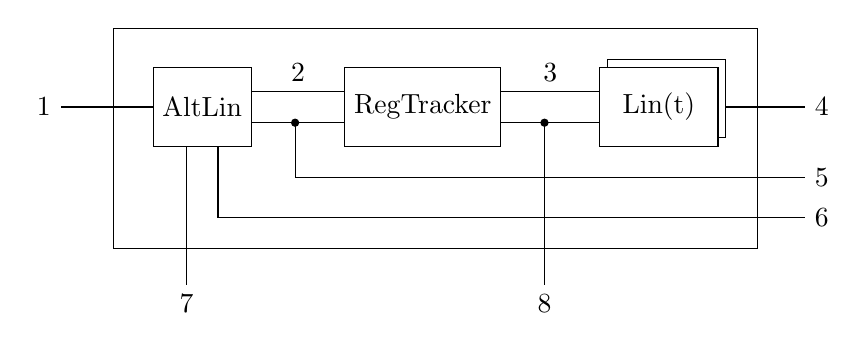
\begin{tikzpicture}
%%%%% AltLin
\draw(0,0) node[draw, minimum height = \height](altSpec){\cspmstyle AltLin};
%% (1)
\draw (altSpec) -- node[left, at end]{\inCircle{1}} ++ (-1.8, 0) 
  coordinate (left); 
%% (7)
\draw (altSpec.south) ++ (-0.2,0) -- node[below, at end]{\inCircle{7}}
   ++ (0,-1.75) coordinate (bottom);
%%%%% RegTracker
\draw (2.8,0) node[draw, minimum height = \height](regTracker){%
  \cspmstyle RegTracker};
%% Syncs between AltLin and RegTracker
\path (altSpec.east) -- ++(0,-0.2) coordinate (a) -- ++(0,0.4) coordinate (aa);
\path (regTracker.west) -- ++(0,-0.2) coordinate (b) -- 
  ++(0,0.4) coordinate (bb);
% (2)
\draw (aa) -- node[above]{\inCircle{2}} (bb);
%%%%% Lin
\draw (regTracker) ++ (3,0) 
  node[draw, minimum height = \height, minimum width = \linW](lin){
    \cspmstyle Lin(t)};
\draw (lin.north west) ++ (\gap, 0.0) |- ++ (\linW, \gap) |- 
  ++ (-\gap, -\height);
%% External coms
%% (4)
\draw (lin.east) ++ (0.1,0) -- node[right, at end]{\inCircle{4}} ++ (1.0,0)
coordinate (right);
%% (6)
\draw (altSpec.south) ++ (0.2,0) -- ++ (0,-0.9) coordinate (temp) -- 
  node[right, at end]{\inCircle{6}} (temp -| right); % (c);
%% (5)
\draw (a) -- (b);  
\fill  (a) ++ (0.55,0) circle(1.5pt) coordinate (t1);
\draw (t1) -- ++ (0,-0.7) coordinate (temp) --
  node[right, at end]{\inCircle{5}} (temp -| right); 
%% (9)
%% \draw (lin.south) -- node[below, at end]{\inCircle{9}}  (lin.south |-bottom);

%% Syncs between RegTracker and Lins
%% (3)
\path (regTracker.east) -- ++ (0,0.2) coordinate (l1) -- 
  ++(0,-0.4) coordinate (l2);
\path (lin.west) -- ++ (0,0.2) coordinate (r1) -- 
  ++(0,-0.4) coordinate (r2);
\draw (l1) -- node[above]{\inCircle{3}} (r1);
%% (8)
\draw (l2) -- (r2);
\fill (l2) ++ (0.55,0) circle(1.5pt) coordinate (temp);
\draw (temp) -- node[below, at end]{\inCircle{8}} (temp |- bottom);
%%%%% Outer box
\path (altSpec.west) -- ++ (-0.5,1) coordinate (a) -- ++(0,-2.8) coordinate (d);
\path (lin.east) --  ++(0.5,1) coordinate (b) -- ++(0,-2.8) coordinate (c);
\draw (a) -- (b) -- (c) -- (d) -- (a);
\end{tikzpicture}
\end{center}

%%%%%%%%%%%

\textbf{Key.} The interface with the alt-thread appears on the left; the
interface with channels appears on the right; error events and spurious
wakeups appear below; internal events appear inside the box.  

\raggedright
%
\begin{itemize}
\item[\inCircle{1}:] \CSPM{(begin}\m\CSPM{end)Alt};

\item[\inCircle{2}:] \CSPM{beginRegistration}, \CSPM{endRegistration},
  \CSPM{getToDeregister(In}\m\CSPM{Out)}, \CSPM{deregisterDone},
  \CSPM{endWait}; 

\item[\inCircle{3}:] \CSPM{maybe(Send}\m\CSPM{Receive)}, \CSPM{portClosed};

\item[\inCircle{4}:] \CSPM{(begin}\m\CSPM{end)Maybe(Send}\m\CSPM{Receive)},
  \CSPM{(begin}\m\CSPM{end)PortClosed}; 

\item[\inCircle{5}:] \CSPM{endRegister(In}\m\CSPM{Out)},
  \CSPM{endDeregister(In}\m\CSPM{Out)};   

\item[\inCircle{6}:] \CSPM{beginRegister(In}\m\CSPM{Out)},
  \CSPM{beginDeregister(In}\m\CSPM{Out)};   

\item[\inCircle{7}:] \CSPM{spuriousWakeup.AltThread}; 

\item[\inCircle{8}:] \CSPM{maybe(Send}\m\CSPM{Receive)Error}, 
  \CSPM{portClosedError}.

%% \item[\inCircle{9}:] \CSPM{spuriousWakeup.t}.
\end{itemize}
%
\caption{Construction of the idealised alt.  \label{fig:idealised-alt}}
\end{figure}

%%%%%%%%%%

\framebox{**} Rename beginRegister, endRegister

The idealised alt is constructed from several components, as depicted in
Figure~\ref{fig:idealised-alt}.  The component |ChanState| keeps track of
registrations of the alt at ports, or whether those ports are closed.  Each
component |Lin(t)| linearises callbacks by channel-thread~|t|.  The component
|RegLin| linearises the main call of the alt by the alt-thread.  We describe
these in more detail below.

%%%%%%%%%%

\begin{figure}
\begin{cspm}
Lin(t) = 
  beginMaybeReceive.t?index?x -> LinMaybeReceive(t, index, x)
  [] beginMaybeSend.t?index -> LinMaybeSend(t, index)
  [] beginPortClosed.t?index -> LinPortClosed(t, index)
  
LinMaybeReceive(t, index, x) = 
  maybeReceive.t.index.x?res -> endMaybeReceive.t.res -> Lin(t)
  [] maybeReceiveError.t.index -> STOP
  
LinMaybeSend(t, index) = 
  maybeSend.t.index?res -> endMaybeSend.t.res -> Lin(t)
  [] maybeSendError.t.index -> STOP
  
LinPortClosed(t, index) = 
  portClosed.t.index -> endPortClosed.t -> Lin(t)
  [] portClosedError.t.index -> STOP
\end{cspm}
\caption{Definition of the {\scalastyle Lin(t)}
  processes.  \label{fig:alt-lin}} 
\end{figure}

%%%%%%%%%%

The |Lin(t)| processes, which linearise the callbacks by thread~|t| from
channels, are defined in Figure~\ref{fig:alt-lin}.  Each callback function is
handled by a different subsidiary process.  Each may be either linearised
correctly, or with an error event if it breaks the alt protocol: The
|RegTracker| process selects the appropriate event, based on whether the alt
is currently registered at the relevant port.  

%%%%%%%%%%

\begin{figure}
\begin{cspm}
AltLin = beginAlt.AltThread -> beginRegistration -> Register(0)
  
Register(i) = 
  if i == size then endRegistration?ac -> 
    if ac then endAlt.AltThread.AltAbort -> AltLin else Waiting
  else Register1(i, nth(branches, i))
  
Register1(i, InPortBranch.c) = 
  beginRegisterIn.AltThread.c.i -> (
    endRegisterIn.AltThread.c.RegisterSuccess?x -> Deregister(AltReceive.i.x)
    [] endRegisterIn.AltThread.c.RegisterWaiting -> Register(i+1)
    [] endRegisterIn.AltThread.c.RegisterClosed -> Register(i+1)
  )

Register1(i, OutPortBranch.c) =
  beginRegisterOut.AltThread.c.i -> (
    endRegisterOut.AltThread.c.RegisterSuccess?x -> Deregister(AltSend.i.x)
    [] endRegisterOut.AltThread.c.RegisterWaiting -> Register(i+1)
    [] endRegisterOut.AltThread.c.RegisterClosed -> Register(i+1)
  )
  
Deregister(result) =
  getToDeregisterIn?c.i -> beginDeregisterIn.AltThread.c.i -> 
     endDeregisterIn.AltThread.c -> Deregister(result)
  [] getToDeregisterOut?c.i -> beginDeregisterOut.AltThread.c.i ->
     endDeregisterOut.AltThread.c -> Deregister(result)
  [] deregisterDone -> endAlt.AltThread.result -> AltLin
  
Waiting = 
  endWait?result -> (
    if result == AltAbort then endAlt.AltThread.result -> AltLin
    else Deregister(result))
  [] (spuriousWakeup.AltThread -> Waiting |~| STOP)
\end{cspm}
\caption{Definition of the {\scalastyle AltLin}
  processes.  \label{fig:AltLin}} 
\end{figure}

%%%%%%%%%%

The |AltLin| process, which linearises the main calls of the alt, is defined
in Figure~\ref{fig:AltLin}.  It is based on a definition |branches| of the
branches of the alt.  It initially signals to the |RegTracker| that it is
beginning registration, via event |beginRegistration|.  It then iterates
through |branches|, trying to register at each branch in turn (the expression
|nth(branches, i)| gives the branch at index~|i|).  The |RegTracker| keeps
track of the results of the registration attempts.  If a registration is
successful, |AltLin| moves to the deregistration phase.  If it gets to the end
of |branches|, it synchronises with |RegTracker| on channel |endRegistration|
to indicates to |RegTracker| that registration is over.  |AltLin| receives
from |RegTracker| a boolean, denoted |ac|, that indicates whether all ports
have been closed; if so, the call on the alt returns with an |AltAbort|;
otherwise, the |AltLin| moves to the waiting phase.

The deregistration phase is defined by the process |Deregister(result)| (where
|result| will be the result of the call of the alt).  It repeatedly gets from
|RegTracker| information about a port to be deregistered, calls the relevant
deregistration function, and waits for it to return.  When there are no more
ports to deregister, |RegTracker| signals this on |deregisterDone|, at which
point |AltLin| ends the call on the alt. 

